\section{Tooling} \label{sec:dsl-implementation}

To validate our approach, we have implemented a tool chain to ease the definition of customized memory profilers for Java-based systems.~\footnote{Available at: \url{https://github.com/intigonzalez/heapexplorer\_language}}
These profilers can be executed in any JVM as long as it provides support for the JVMTI.

In this section, we present tools built to support the definition of memory profilers using our language; this is done by taking into account how engineers in different roles may interact with these tools and with the resultant profilers.
Indeed, in dealing with memory profilers, we have to take into consideration the two usual roles -- developers of profilers and their users; after all, profilers built using our language are themselves software abstractions.
A developer must know how the target domain-specific abstractions are represented on top of the JVM, and she/he must also have a clear understanding of how our language is executed.
On the contrary, users only need to be aware of the interface provided by our framework, and the structure of the data collected by a profiler.
In the rest of this section, we discuss details that are important to these roles.

In this section, we also present low-level details regarding how the language is implemented on top of the JMVTI.
The decision of implementing our approach by relying on JVMTI has advantages and disadvantages.
On the one hand, the obvious advantage lies on the portability of this solution, which makes it more valuable from a practical point of view.
On the other hand, building profilers on top of the JVMTI; instead of directly modifying the JVM, impacts the performance of the generated profilers and, unfortunately, hinders (in extreme case it even prevents) the implementation of some language constructs.
Nonetheless, it is our belief that guaranteeing profilers' portability should be of maximum priority.
Moreover, in writing this implementation, we have found that the limitations in the JVMTI preventing the construction of better profilers can be overcome with, at most, a few additions to the API.


\subsection{Developers of domain-specific abstractions}

%\extracomment{FIX}{I am fixing this section, you can continue in Section~\ref{sec:dsl-tooling-users}}

In our vision, developers of software libraries and component frameworks, as well as software language engineers may use our approach to  define customized memory profilers for the abstractions they create.
This is, in addition to delivering artifacts such as libraries, source code, simulators, text editors for DSLs, and compilers for these DSLs; engineers would also ship profilers to simplify the use of these abstractions.
For instance, the developers of the Spring framework~\footnote{\url{https://spring.io/}} may create a set of specific profilers to reduce the cost of maintaining applications written using the framework.
These profilers can serve as both internal tools to help in the development of abstractions, and mechanisms allowing users to better use abstractions.

Figure~\ref{fig:dsl-tooling-developer} summarizes the viewpoint of developers of domain-specific abstractions.
To write a profiler, they use knowledge about the abstraction and the tool chain to generate the executable profiler. 
Our implementation of the language is built using Xtext~\cite{Eysholdt:2010:XIY:1869542.1869625}; it provides a textual editor that is able to handle the proposed concrete syntax.
This editor provides syntax highlighting, error detection during editing, auto-completion, and compilation to native Java agents written in \textit{C++}.

\begin{figure}
\centering
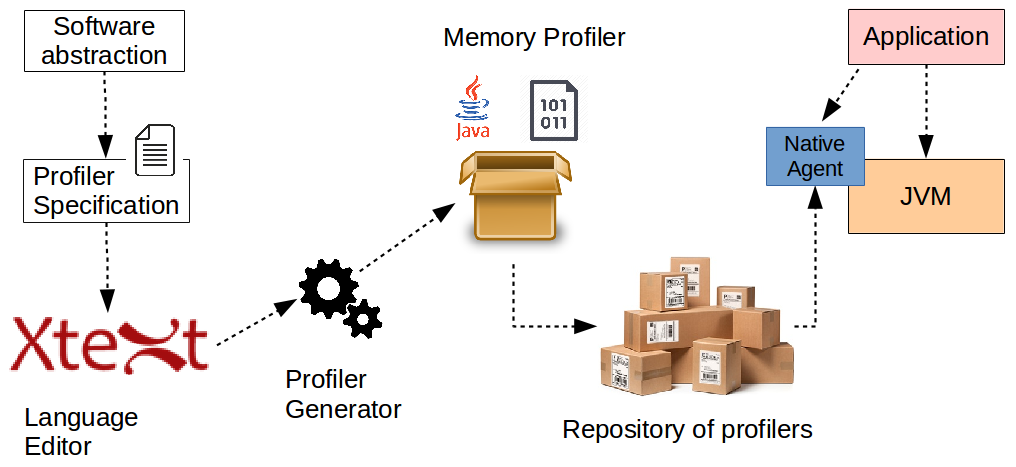
\includegraphics[scale=0.45]{./chapter6/fig/developer-profiler-view.png}
\caption{Developer viewpoint. Memory profilers are built from the description of software abstractions.}\label{fig:dsl-tooling-developer}
\end{figure}

To perform low-level tasks related to memory profiling, we use \glslink{JVMTI}{JVMTI}~\footnote{\url{http://docs.oracle.com/javase/8/docs/platform/jvmti/jvmti.html}} and \glslink{JNI}{JNI}.
These APIs are used by both profilers and the core memory profiling library, so-called Native Agent in Figure~\ref{fig:dsl-tooling-developer}.
In this native agent, a \textit{plugins} system, which allows users to load/unload profiles without shutting down the JVM, is implemented.
Given a profiler definition, the compiler output is a package that contains the native binary code for the profiler, and a Java library you can use to access the collected data using plain Java objects.

To reduce the overhead of profilers, developers must be aware of the details of the abstraction for which the profiler is being built, the semantic of our language, and the details of its implementation.
In particular, it is advisable reducing the usage of \textit{lists} and the evaluation of nested lambda expressions.
Likewise, heavily using the built-in rvalue \textit{objects} is especially discouraged because it can easily contain many elements.
It is also discouraged because, in order to reduce memory consumption, we rely on an iterator built on top of JVMTI operations that can be costly to use in terms of CPU time.

Finally, we added some built-in rvalues in this implementation because they are both useful in the context of Java and easy to obtain using the JVMTI.
These values are \textit{classes}, \textit{classloaders}, \textit{threads} and \textit{objects}; they are lists of anonymous built-in record types.
The relation among these types and their operations are depicted in Figure~\ref{fig:dsl-built-in-types}.

\begin{figure}
\centering
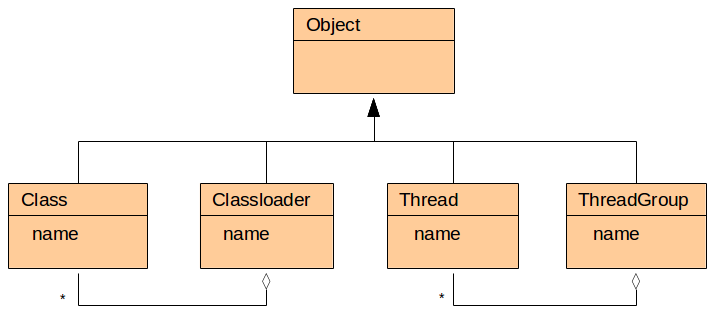
\includegraphics[scale=0.45]{./chapter6/fig/diagram-classes.png}
\caption{Viewpoint of developers. Memory profilers are built from the description of software abstractions.}\label{fig:dsl-built-in-types}
\end{figure}

%Indeed, the process of code generation is driven by the need of reducing the performance impact.
%In our implementation, we apply a set of platform dependent optimizations taking into account the profiler description.
%First, since a profiler does not always need built-in rvalues (e.g., \textit{threads}, \textit{threadgroups} and \textit{classes}, etc.), we selectively skip the construction of them.
%When possible, we also skip the construction of some structures (e.g., class of each object, its classloader, field names, etc.).

\subsection{Users of domain-specific abstractions} \label{sec:dsl-tooling-users}

We envision that a set of memory profilers can be shipped in addition to other ``classic'' deployment artifacts that users of a software abstraction receive. 
These profilers would support the use of the corresponding software abstraction.
For instance, a user who is relying on a new extension of the Xtend language to build a system, may use specific profilers written in our language to understand the memory consumption, and in general, the behavior of the system.

The generated profilers can be used in two different ways, either as development tools or as mechanisms to support resource awareness at runtime.
Due to the scope of this thesis, the reference implementation we provide is biased towards the second scenario, but it should be relatively simple to adapt it to support the software development process.
To access memory profilers, a JVM must be launched with a native Java agent loaded, and a library to collect profiling data in its classpath.
Once the application is running, it can trigger profiling by simply issuing a few method calls using the profiling API.
Figure~\ref{fig:user-profiling-library-view} illustrates the process of collecting memory profiles, the software components involved, and the APIs that must be used.
Observe how the profiling framework issues a call to a handler once it is done, a parameter contains the data computed.
These data are encoded in a \textit{list}, in which each elements correspond to the data computed for each identified structure in the heap.
%The problem is knowing the type and shape of each list element.

\begin{figure}[!t]
\centering
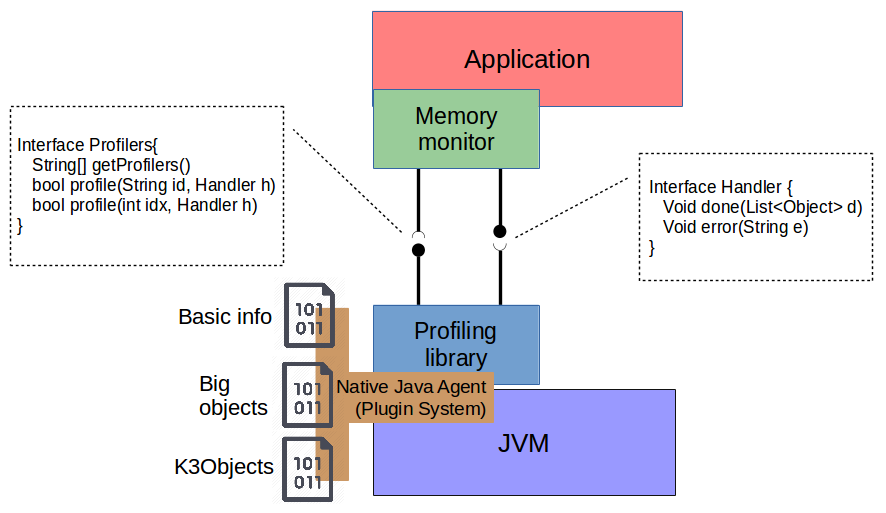
\includegraphics[scale=0.5]{./chapter6/fig/user-profiler-view.png}
\caption{Viewpoint of users. Memory profilers are black-boxes accessed through Java interfaces. Data collected is in the form of plain Java objects.}\label{fig:user-profiling-library-view}
\end{figure}

The output of a profiler is a list of Java objects containing the collected information; and the type of these objects depend on the profiler definition.
Indeed, as part of our implementation, the profiler generator creates a set of Java classes to represent the data collected in a form that is easy to digest at runtime by a Java application.
Once a profiler collects the information in an internal format, it populates a representation in Java using the \gls{JNI}; the code to do so is also generated by the compiler of our language.
In Figure~\ref{fig:dsl-generated-java}, the classes generated for a profiler are shown.
Notice that a class is created for each \textit{record} declared, and also for each \textit{StructureType}.
It can be seen how `lists' are directly represented in Java by mean of generic Java lists.
The \textit{id} field in both \textit{MemoryProfile1} and \textit{MemoryProfile2} is the value used to parametrize each structure.
In this particular example, where two structures are identified, the value of \textit{MemoryProfile1.id} is ``lists'' and the value of \textit{MemoryProfile2.id} is ``otherObjects''.

Given the fact that the data computed by a profiler is returned as a list of objects, and their layout is unclear, the remaining problem is how to process such data; there are two options.
First, users can make the application code depends on the Java code created by the profiler generator.
In this way, your application has a new dependency, but you can profit from knowing at development time the types used in the code.
A second approach is using the reflection capabilities of Java to explore the data.
In the evaluation, we use such an approach to log the result of an arbitrary profiler, printing all the information it has computed.
Using reflection, it is also possible to build a user interface to explore the results in a customized way.  

\begin{figure}
\centering
\begin{minipage}[t]{0.60\linewidth}
\begin{lstlisting}[language=DSL2]
name "basic info" 
T : struct {
	name : String
	size: int
}
create structeres for e:#["lists"]
using
	constructor
		initialObjects = #Object[]
		data1 = #T[];
	membership (this is String) or (this is Array)
	updates
		data1 = data.add(struct T { this.name, this.size})
		
create structeres for e:#["otherObjects"]
using
	constructor
		initialObjects = #Object[]
		data2 = #T[];
	membership true
	updates
		data2 = data.add(struct T { this.name, this.size})
\end{lstlisting}
\end{minipage}
\hspace{0.07\linewidth}
\begin{minipage}[t]{0.30\linewidth}
\begin{lstlisting}[language=java, frame=L, numbers=left,numberstyle=\color{black}\scriptsize]
class T {
	final String name;
	final int size;
}

class MemoryProfile1 {
	final Object id;
	final List<T> data1;
}

class MemoryProfile2 {
	final Object id;
	final List<T> data2;
}
\end{lstlisting}
\end{minipage}
\caption{Representation of profiling data in Java, as users of profilers see it. Accessing these structures is useful to support resource awareness.} \label{fig:dsl-generated-java}
\end{figure}

\subsection{Implementation Details}
Using \gls{JVMTI} and \gls{JNI} to create the built-in values \textit{threads}, \textit{threadgroups}, \textit{classes}, and \textit{classloaders} is simple.
These APIs provide routines that one can use to obtain the information from the JVM.
Since the number of threads (and classes) is relatively small, we simply store the data in a \textit{vector} (included in the \textit{C++} \gls{STL}) to reuse it every time we need it.
On the contrary, creating the built-in value \textit{objects} is challenging.
Indeed, keeping a \textit{vector} with references to all objects is not acceptable in terms of memory consumption because of the large number of objects in the heap.
Fortunately, we can overcome this problem by noticing that iterating over the objects is usually enough to implement the language.
For instance, in Listing~\ref{lst:listLengt} we need to iterate over the objects, and filter an object out if its type is not \textit{SinglyLinkedList}.
When this listing is executed in the memory snapshot shown in Figure~\ref{fig:simple_snapshot}, the result is a \textit{vector} with only two elements.

To iterate over objects, we use the routine ``\textit{FollowReferences}''.
This function basically traverses the reference graph invoking a set of callback functions every time a new reference is found. 
In these callbacks, we generate the code to filter objects.
For examples, Listing~\ref{lst:follow_references} illustrates how is the code generated for the expression:

\begin{lstlisting}[escapeinside={(*}{*)},language=DSL2
]
objects.filter([o | ret o is SinglyLinkedList])
\end{lstlisting}

Notice that accessing an object from within the callback is not possible.
Instead, one can only access a \textbf{tag} associated to the object.
This is the major limitation we find in implementing our language using the JVMTI.
\footnote{This constraint is imposed in the implementation of the JVMTI function ``\textit{FollowReferences}'' because no mutator code can be executed when the reference graph is being traversed. By using tags instead of objects, the JVM guarantees that no JNI function is invoked.}
Likewise, these callbacks offer metadata, such as the class and reference info, that we can leverage.

\begin{lstlisting}[language=C++, frame=L, numbers=left,numberstyle=\color{black}\scriptsize, xleftmargin=1.5\parindent, label={lst:follow_references},
caption={Code generated for the expression \textit{objects.filter}. This is a simplified version in C++14}]

jint references(jvmtiHeapReferenceKind ref_kind,  const jvmtiHeapReferenceInfo* ref_info, 
     jlong class_tag,  jlong referrer_class_tag, 
     jlong size,  jlong* tag_ptr, jlong* referrer_tag_ptr, 
     jint length, void* user_data) {
  ...
  vector<DSL_TAG>* tags = (vector<DSL_TAG>*)(user_data);
  DSL_Class cl = getFromTag(class_tag);
  if (cl.name == "SinglyLinkedList")
	  tags->push_back((DSL_TAG)*tag_ptr);
  ...
}

vector<DSL_OBJECT> v;
vector<DSL_TAG> tags;
callbacks.heap_reference_callback = references;
jvmtiEnv->FollowReferences(NO_FILTER, NULL, NULL, callbacks,&tags);
for (auto f : tags) {
	jlong* a_tags = {f};
	jint count_ptr;
	jobject* object_result_ptr;
	jlong* tag_result_ptr;
	jvmtiEnv->GetObjectsWithTags(1, a_tags, &count_ptr, &object_result_ptr, &tag_result_ptr);
	v.push_back(jobject2DSLObject(object_result_ptr[0]));
}

\end{lstlisting}

An additional mechanism is required when a lambda expression for filtering \textit{objects} is accessing attributes of an object.
For instance, in Listing~\ref{lst:dsl-example1} a primitive attribute, ``\textit{data}'', is accessed, while a reference attribute ``\textit{key}'' is read in Listing~\ref{k3}.
Reading primitive attributes is supported by the JVMTI function \textit{FollowReferences}; by simply supplying the appropriates callbacks,  you can get the value of every primitive field.
However, this is not enough.
The problem is that -- to completely evaluate a lambda expression -- the values involved in the expression must be collected in different execution contexts.

\begin{figure}[!b]
\centering
\begin{minipage}[t]{0.35\linewidth}
\begin{lstlisting}[language=DSL2]
[ o | o.data > 3 and 
	  (referrer is String) and 
	  (o.key is HashMap.Entry)] 
\end{lstlisting}
\end{minipage}
\hspace{0.07\linewidth}
\begin{minipage}[t]{0.55\linewidth}
\begin{lstlisting}[language=java, frame=L, numbers=left,numberstyle=\color{black}\scriptsize]
references_callback() {
	obj_tag = (DSL_TAG)*tag_ptr;
	t0 = referrer_class.name == "String";
	if (!t0) return;
	obj_tag->fun = [=](String a, jvalue v) { 
	  if (a == "data")
	    return t0 && v > 3;
	  return false;
	};
	vector<DSL_TAG>* tags = (vector<DSL_TAG>*)(user_data);
	tags->push_back(obj_tag);
}

primitive_callback() {
	obj_tag = (DSL_TAG)*tag_ptr;
	t2 = obj_tag->fun(field_name, field_value);
	obj_tag->fun = [=]() { 
	  jobject obj = getFromTag(obj_tag); 
	  jobject key = obj.key; // JNI
	  t3 = isInstance(key, "HashMap.Entry");
	  return t3; 
	};
}
\end{lstlisting}
\end{minipage}
\caption{Evaluating an expression through partial evaluation.} \label{fig:dsl-closures}
\end{figure}

The solution we propose is based on using the functional library of \textit{C++11} to implement continuations.
In other words, we build \textit{functions} that contain parts of the evaluation of a lambda expression, the values already computed are stored in the closure associated to the \textit{function}.
Figure~\ref{fig:dsl-closures} shows the transformation of an expression.
Observe how it requires collecting data in two different places, and partially evaluating the expression in three places.

Unfortunately, our solution has limitations.
For instance, it cannot handle nested uses of the built-in value \textit{objects} nor access primitive attributes of the referrer object.
Indeed, so far we have discussed how to evaluate expressions that involve the list of \textit{objects}, but evaluating the membership and update functions are problem with a similar solution.
In other words, we also use the function \textit{FollowReferences} to identify the \textit{structures} in the heap.

We perform some optimizations related to the construction of the built-in values \textit{threads}, \textit{threadgroups}, \textit{classes}, etc. 
Since not all memory profilers depends on such values, we selectively skip the construction of them.
We also extend this to other cases. For instance, we do not find the class of each object when it is not required, and we avoid processing classes to obtain field names when they are not used in an expression.
To implement these optimizations, we used a parametrized code template; therefore, the generated code depends on the values of generic parameters. 
We can tune them to satisfy our needs.
Another optimization is reducing the number of nodes that must be traversed.
As an illustration, we only produce code to explore primitive fields of each object, which are represented as leaf nodes in the graph, if there exists an expression accessing a field.


%The process of code generation is driven by the need of reducing the performance impact.
%In general, there are two ways of optimizing the impact of the memory's analysis.
%First, we can apply platform dependent optimizations.
%The second option is to apply platform independent optimizations; for instance, simplifying the evaluation of each expression.
%In our implementation, we use both platform dependent and independent optimizations.
%
%A set of platform dependent optimizations we perform is related to the construction of the built-in values \textit{threads}, \textit{threadgroups}, \textit{classes}, etc. 
%Since not all memory analysis depends on such values, we selectively skip the construction of them.
%For instance, in listing~\ref{assertion} there is no need to compute any of such values as is also unnecessary to identified the class of each object.
%Extending this idea to other cases (e.g., class of each object, its classloader, field names, etc.) is straightforward.
%To implement these optimizations, we used a parametrized code template, so the code generate depends on the values of these parameters which we can tune to satisfy our needs.
%
%An other optimization we perform is related to the existence of collections as data type in our DSL.
%These collections can be potentially large, in particular, the \textit{objects} value is costly to compute and keep in memory.
%This fact combined with the usage of operations on collections such as \textit{map} and \textit{filter} may harm the performance of an analysis.
%That is why we devise two strategies to deal with collection values.
%User-defined and most built-in collections are kept in memory using linear space.
%On the contrary, we represent the built-in collection \textit{objects} as a generator.
%This representation is feasible because the mechanism provided by JVMTI to access the objects is based on callbacks.
%
%A last optimization is reducing the nodes of the graph that must be traversed
%As an illustration, we only produce code to explore primitive fields of each object, which are represented as leaf nodes in the graph, if there exist some expression accessing a field.
%
%As for platform independent optimizations, we mostly change the order in which boolean expressions are evaluated.
%We try to guarantee that subexpressions accessing collections and fields are evaluated as little as possible.
%
%The current implementation is limited in the number of optimization it applies.
%The main overhead reduction is achieved thanks to the execution model in which many paths of the graph are not traversed.
%Other benefits come from deciding at compilation time if some parts of the graph such as the leaf nodes must be explored or not.
